\chapter{Creating SD-card}

\section{Introduction}

This chapter describes how to create a SD-card that will boot on your picosafe.

\section{Creating partition table and LUKS container}

If you just want to create a SD-card with a running linux system, you may use
the script \texttt{genrootfs.sh} in the directory \texttt{rootfs/}. This script
will perform following steps:

\begin{enumerate}
\item Filling the SD-card with random data.
\item Creating the partition table and the filesystems.
\item Creating a LUKS container with a ext3 filesystem.
\item Copying the linux root filesystem to the LUKS container.
\item Copying the linux kernel modules to the LUKS container.
\item Copying the linux kernel to the SD card.
\item Copying the apex bootloader to the SD card.
\end{enumerate}

To create a SD-card, run:

\texttt{\$ cd rootfs} \\
\texttt{\$ sudo ./genrootfs.sh /dev/sdX keyXX\_picosafe.key \[PEM_FILE\]}

where \texttt{/dev/sdX} is the block device of your SD-card. You may specify a
\texttt{PEM\_FILE} that will be used for the webserver. If omitted, the file
will be generated.

The default password for the LUKS container is \texttt{picosafe}.

\section{Partition table}

This section gives aditional information on the partition table and how to
create it yourself. So you usually can just skip this section.

\begin{wrapfigure}{r}{0.5\textwidth}
  \begin{center}
    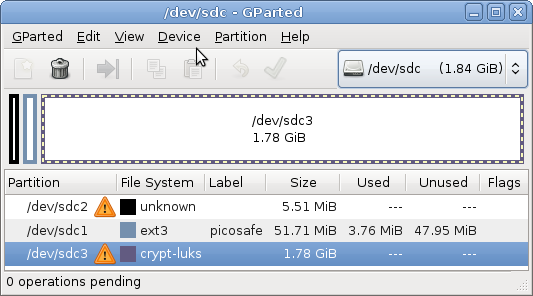
\includegraphics[width=0.5\textwidth]{gparted.png}
  \end{center}
  \caption{Partition table of SD-card shown by gparted.}
\end{wrapfigure}

The SD-card must contain three primary partitions: A bootit (id \texttt{0xDF})
partition with size of a few megabytes that contains the apex bootloader, a
partition formated with ext3 (id \texttt{0x83}) that contains the kernel, and a
partition that contains the LUKS container with the root filesystem. The
bootit partition must be physically the first partition on the SD-card, i.e.
it must start after partition table. It is recommended that the bootit
partition is (logically) the second primary partition, and the ext3 partition
with the kernel is the first primary partition. The bootit partition should
have a size of few megabytes, the ext3 partition should use about 50 megabytes.
The last partition for the LUKS container should use all the space left on the
SD-card.

If you want to create the partition table yourself, you may use your favourite
tool or you may use the script \texttt{partition.sh} in the directory
\texttt{rootfs}. This script will use fdisk to create the partition table and
format the ext3 filesystem. You only need to pass the blockdevice of the
SD-card to the script. As you are writing to a block device, you will need root
privilidges. Also make sure that your are giving the right block device as
argument to the script. Be carefull, as this may destroy any data on the block
device! Also make sure that there is no partition of the SD-card mounted when
executing the script.

\texttt{\$ cd rootfs} \\
\texttt{\$ sudo ./partition.sh /dev/sdX}

\section{Copying kernel}

Mount the ext3 filesystem of the SD-card and copy the encrypted kernel to it
(see chapter Compiling kernel).

\texttt{\$ sudo mount /dev/sdX1 /mnt} \\
\texttt{\$ sudo picosafe\_aes -k key.txt -o /mnt/zImage.crypt zImage}

\section{Copying apex bootloader}

In order to copy the apex bootloader to the bootit partition of the SD-card, you
may use the \texttt{dd} command. Be sure to pass the correct block device as
\texttt{dd} will overwrite any existing data.

\texttt{\$ sudo dd if=../bootloader/apex.rom of=/dev/sdX2}
